\documentclass[11pt,letterpaper]{article}
\usepackage[lmargin=1in,rmargin=1in,tmargin=1in,bmargin=1in]{geometry}
\usepackage{../style/homework}
\usepackage{../style/commands}
\setbool{quotetype}{true} % True: Side; False: Under
\setbool{hideans}{true} % Student: True; Instructor: False

% -------------------
% Content
% -------------------
\begin{document}

\homework{1: Due 01/25}{I mean not homework. It's not work if you love it.}{Alex Dunphy, Modern Family}

% Problem 1
\problem{10} \textit{High Voltage} is an electronics store that, among other products, sells televisions. They sell a particular brand of OLED TV that costs \$949.99. To help drive up sales, they will place the TV on sale for 15\% off. 
	\begin{enumerate}[(a)]
	\item What is the mark-down on this television, i.e. what is the discount?
	\item What is the final advertised price for the television?
	\item How much is the TV after a sales tax of 7\%. 
	\item Suppose over next two months, they discount the price by 15\% twice, what is the advertised price of the television? 
	\end{enumerate}



\newpage



% Problem 2
\problem{10} Suppose that Richard Hoover is driving across the Southwest. After a day of driving, he maps out his travel plans over the next few days. He predicts that the total number of miles he will drive $d$ days from now is given by $M(d)= 390d + 135$. 
	\begin{enumerate}[(a)]
	\item What is the slope of $M(d)$? What does it represent?
	\item What is the $y$-intercept of $M(d)$? What does it represent?
	\item On the plot below, sketch $M(d)$. 
	\item Find how many miles he will have driven after 3 total days of driving.
	\end{enumerate}
	
	\vfill
	
	\[
	\fbox{
	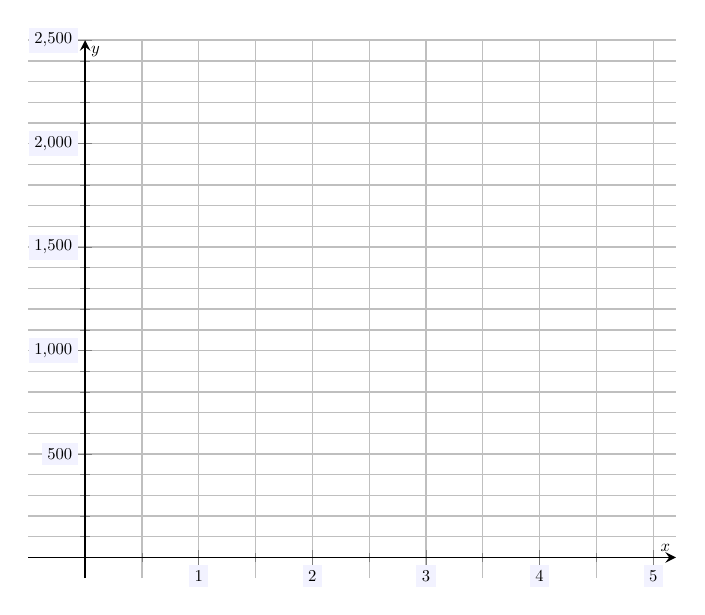
\begin{tikzpicture}[scale=1.2,every node/.style={scale=0.5}]
	\begin{axis}[
	grid=both,
	axis lines=middle,
	ticklabel style={fill=blue!5!white},
	xmin= -0.5, xmax=5.2,
	ymin= -100, ymax=2500,
	xtick={0,1,2,3,4,5},
	ytick={0,500,1000,...,2500},
	minor x tick num = 1,
	minor y tick num = 4,
	xlabel=\(x\),ylabel=\(y\),
	]
%	\addplot[domain=-10.5:10.5,samples=2,line width=0.03cm] (x, 3/5*x - 3);
	\end{axis}
	\end{tikzpicture}
	}
	\] 


\end{document}